\documentclass[11pt]{beamer}

%%% \mode must be on a line by its own, without comment or whitespace!
%%% \mode sets the mode to presentation. So if the mode is presentation the slides after are shown
%%% if the mode is not presentation (but article or handout) they are not shown
\mode<presentation>{}

\usetheme{Warsaw}
\usepackage[utf8]{inputenc}
\usepackage[english]{babel}
\usepackage{amsmath}
\usepackage{amsfonts}
\usepackage{amssymb}
\usepackage{graphicx}
\usepackage{xspace}

\author{Guus Bonnema}
\title{Final Presentation\\(XMas Designer)}
%\setbeamercovered{transparent} 
%\setbeamertemplate{navigation symbols}{} 
%\logo{} 
\institute{Open University\\team033\\Guus Bonnema, Stefan Versluys, Jeroen Kleijn} 
\date{May 20, 2015} 
\subject{XMas Designer} 

\begin{document}

\newcommand{\Noc}{\textsc{NoC}\xspace}
\newcommand{\qt}{\textsc{Qt}\xspace}
\newcommand{\qml}{\textsc{Qml}\xspace}

\begin{frame}
\titlepage
\end{frame}

\begin{frame}{Assignment}
	\begin{itemize}
		\item Create a platform independent, maintainable application to develop
			  a Network on Chip (NoC)
		\item Refactor or rewrite the current application
	\end{itemize}
\end{frame}

\begin{frame}{Overview Process}
	\begin{columns}
		\begin{column}[t]{5cm}
			Process
			\begin{itemize}
				\item <1->Planning phase: DAD approach
				\item <1->Domain analyses
				\item <1->Iteration 0 Architecture
				\item <1->Iteration 1 Build procedures and first prototype
				\item <1->iteration 2, 3, 4, 5 software development
				\item <1->\textit{Final Demo}$\leftarrow$
				\item <1->\textbf{transition}
				\begin{itemize}
					\item {\tiny research context}
					\item {\tiny software release version}
					\item {\tiny final presentation}
				\end{itemize}
			\end{itemize}
		\end{column}
		\begin{column}[t]{5cm}
			Development factors
			\begin{itemize}
				\item <2,7->Time boxing
				\item <3,7->Early switch to \qt
				\item <4,5,7->UI design : \qml
				\item <5,7->Qml / xmas integration: fat interface
				\item <6,7->Reorg OU $\rightarrow$ Communication drop
			\end{itemize}
		\end{column}
	\end{columns}
\end{frame}

\begin{frame}{Contribution to research project}

	\begin{itemize}
		\item support for papers to reason about verification tools of NoC
		\item support for designs of NoC
		\item support for developers and testers of verification tools
		\item support for marketing of research efforts at OU and Radboud university
	\end{itemize}

\end{frame}

\begin{frame}{Example NoC}

\end{frame}

\begin{frame}{Demo XMAS Designer}
	Demo : how? Who will do it? how long? Prerecorded?
\end{frame}

\begin{frame}{Specification model Data Layer iteration 1}

	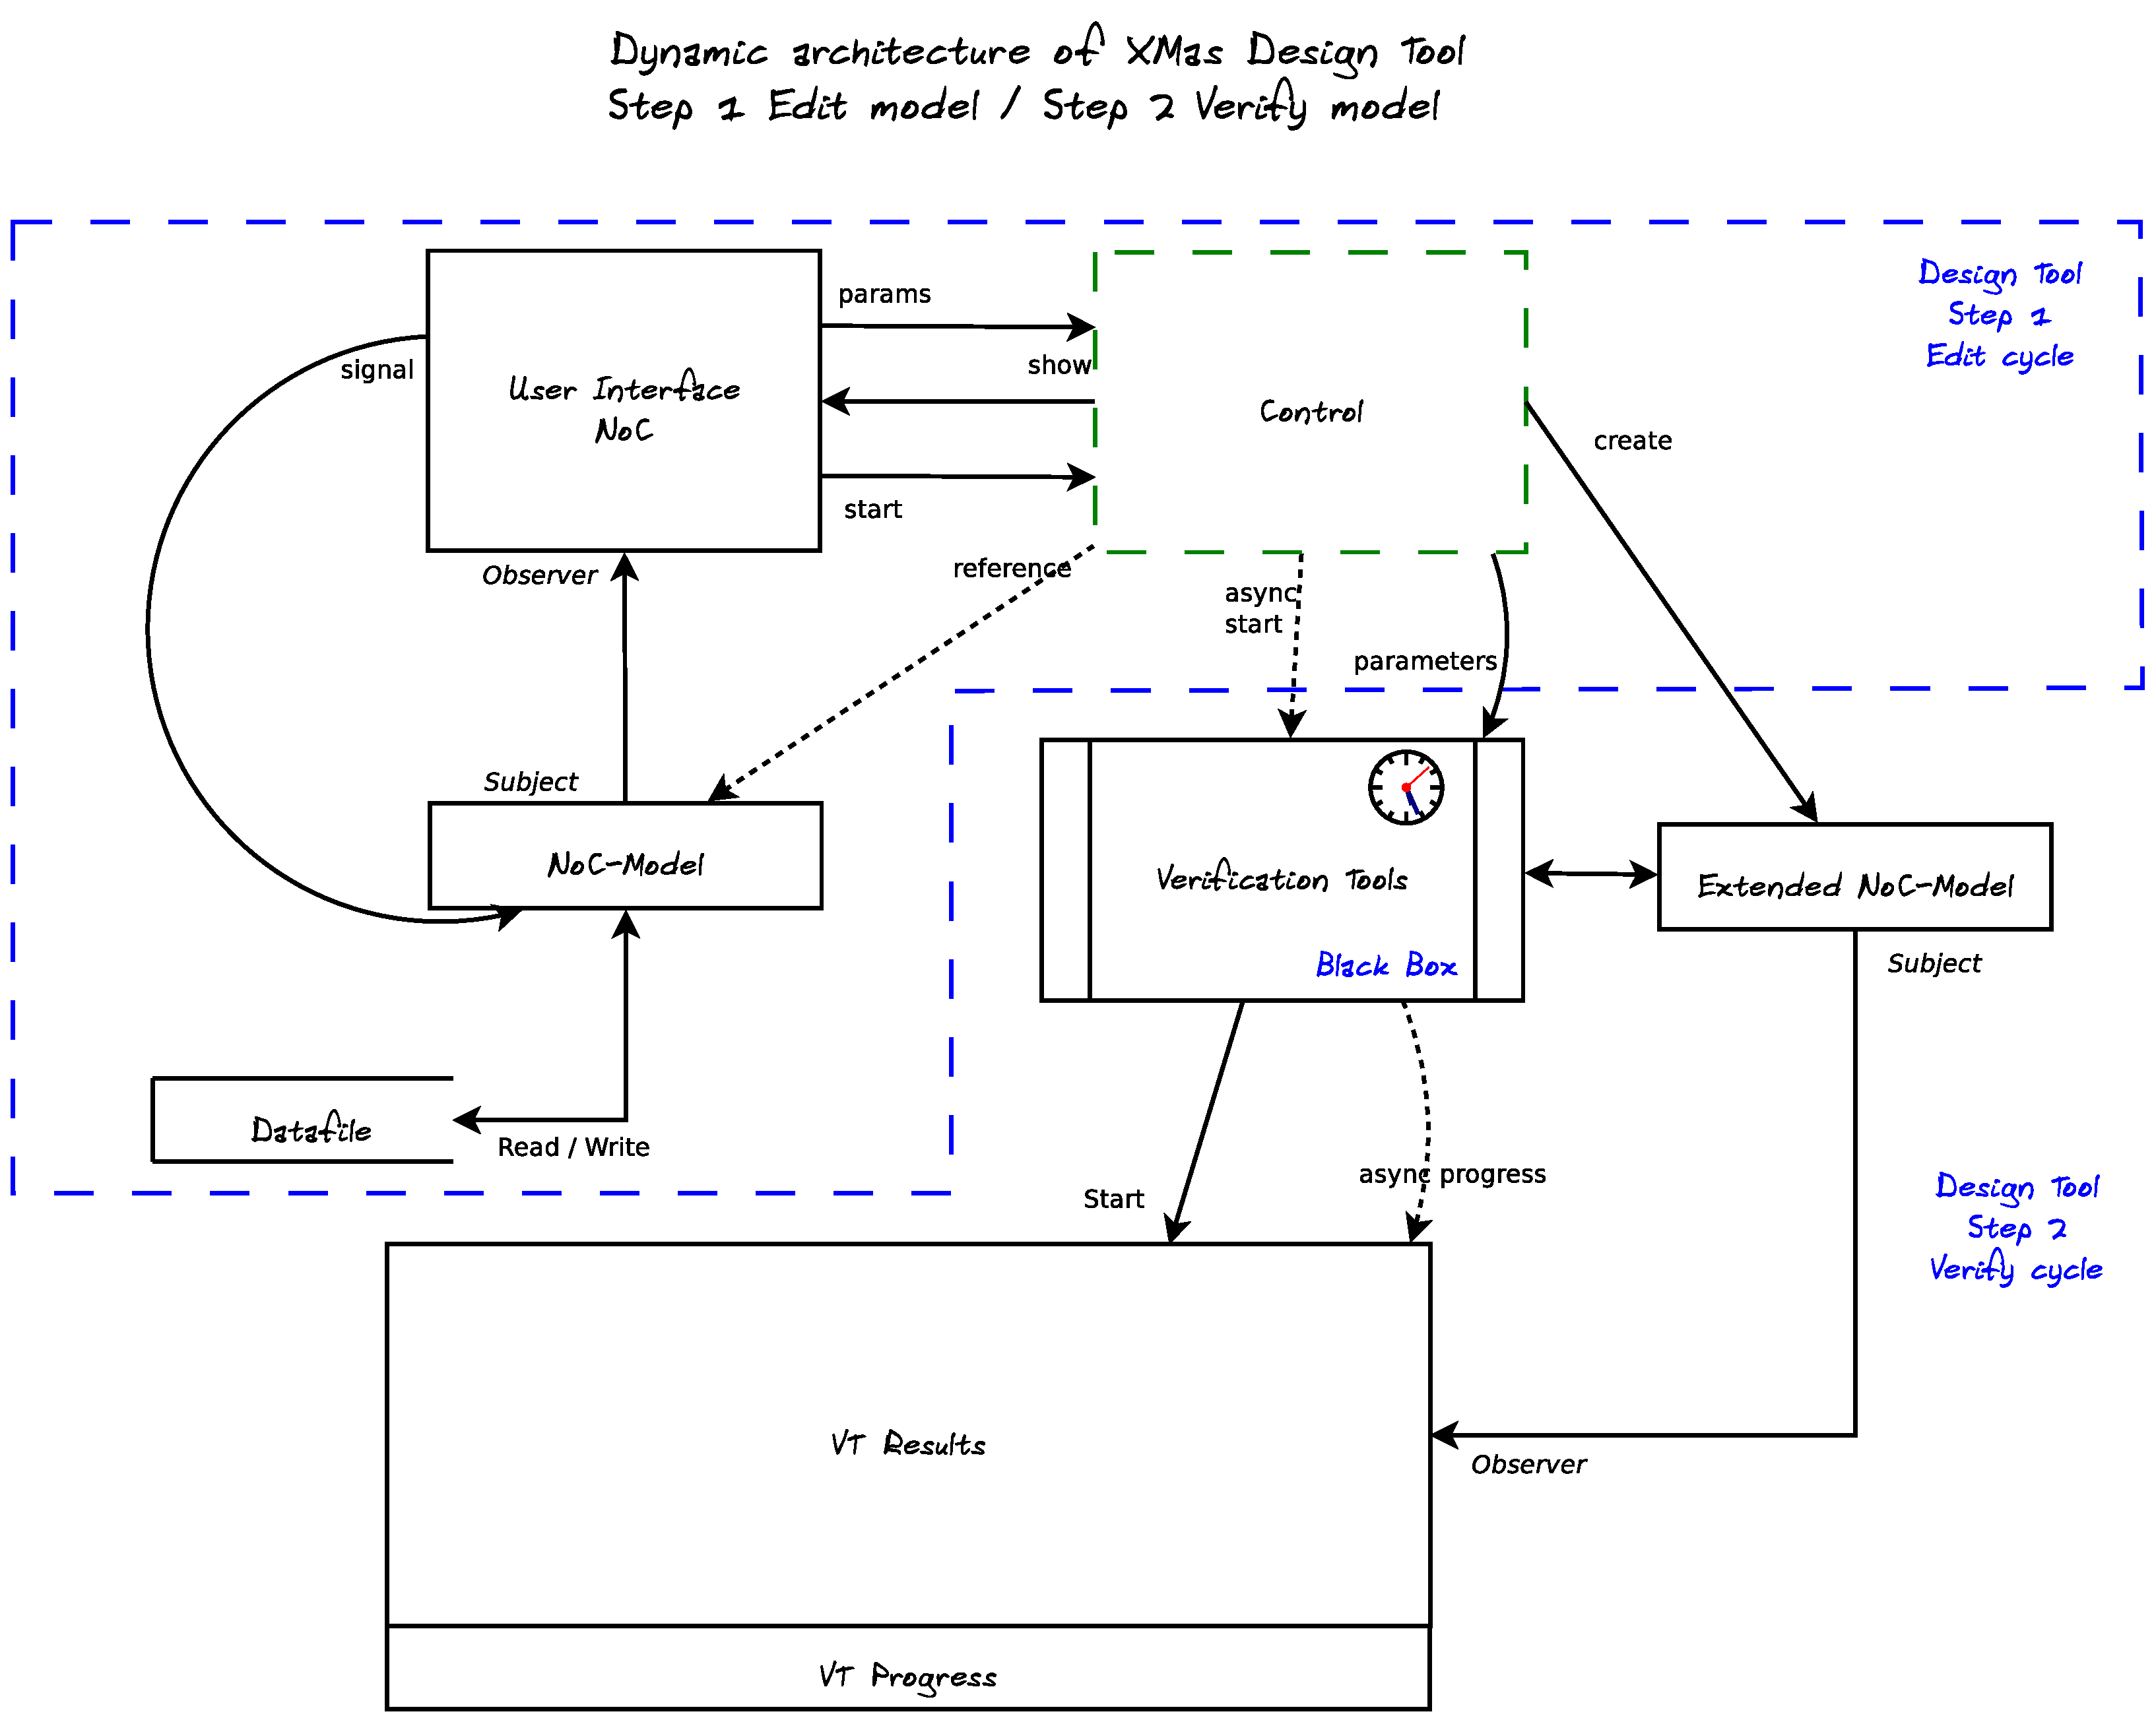
\includegraphics[width=.95\linewidth]{pictures/1c-architecture-dynamic-1}

\end{frame}

\begin{frame}{Implementation Data layer}

	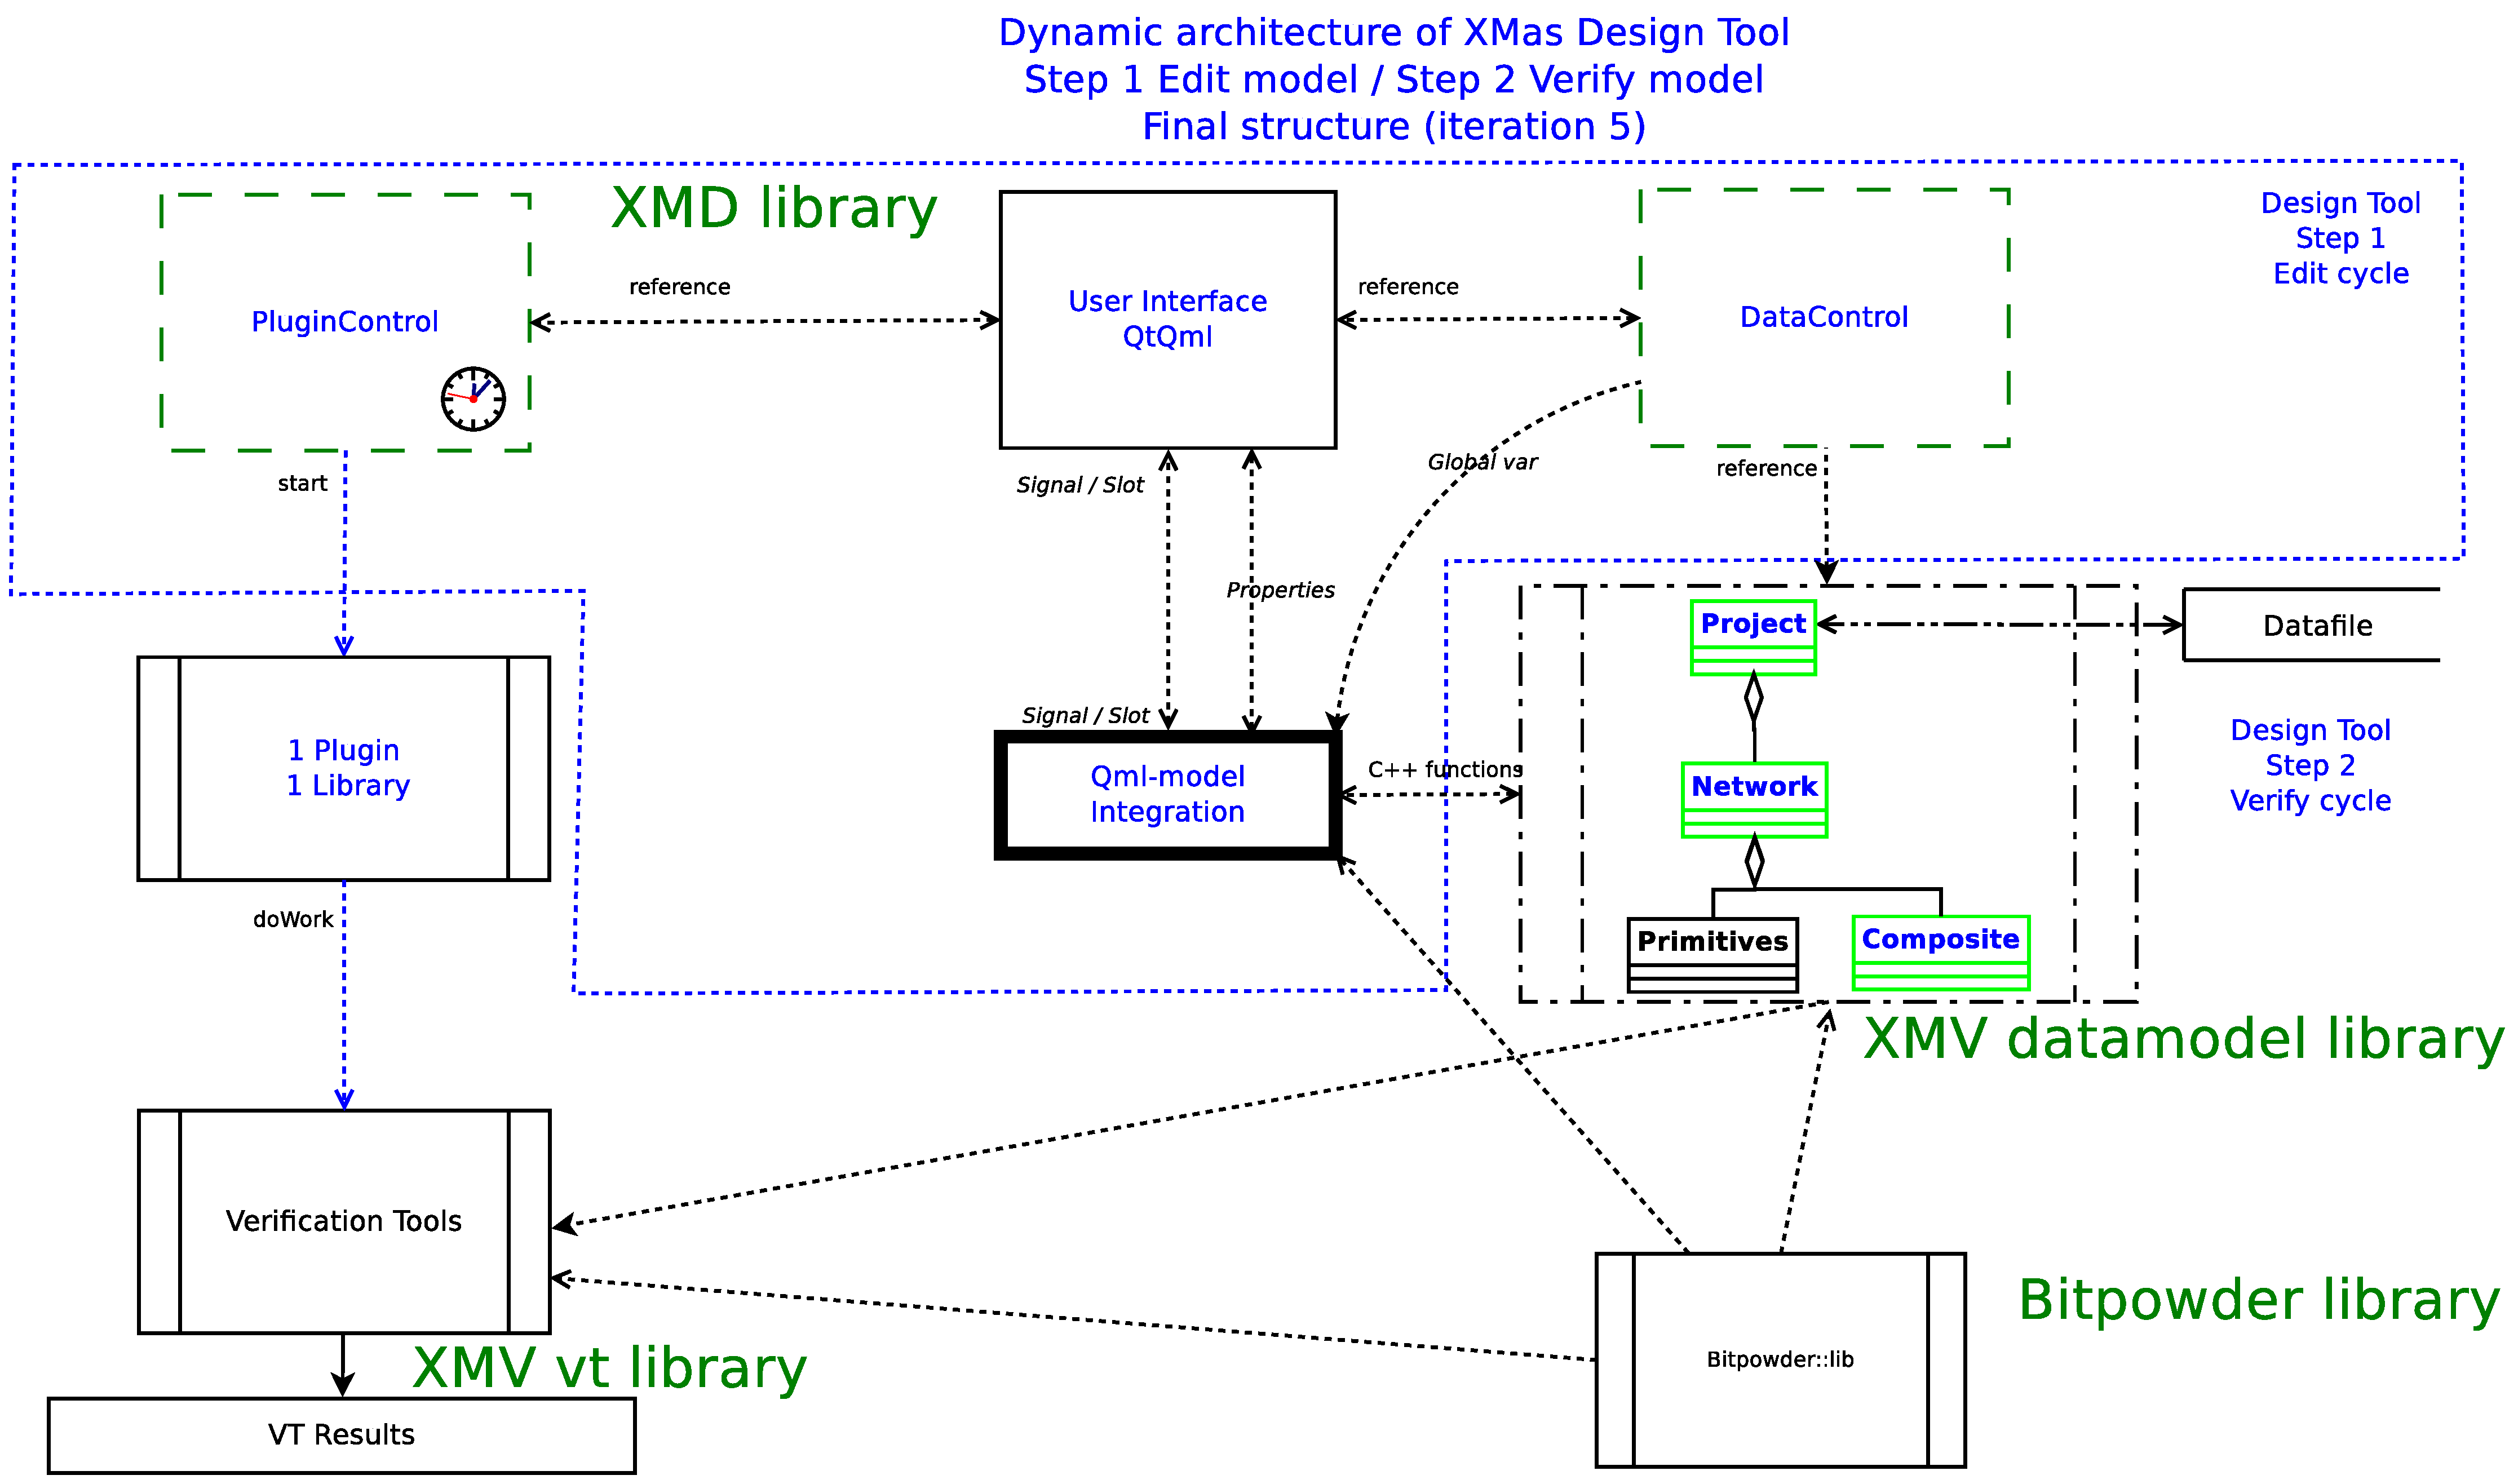
\includegraphics[width=.95\linewidth]{pictures/1c-architecture-dynamic-2}

\end{frame}

\begin{frame}{Project Reflection}
	\begin{itemize}
		\item {\bf Working agile} was evidently the way to do this project. Up front
				we had no idea what to expect and how easy it would be. So we agreed
				to time boxing, using tools like skype, teamviewer, and, Agilefant, github.
				There was no one tool to provide all at the required quality.
				The approach could withstand the attack made by OU reorganization. Although we
				did (internally) discuss replanning, we didn't.
		\item {\bf Planning} We followed the planning exactly. One adjustment for OU reorganization: modifed one risk
				and added one measure.
		\item {\bf Cooperation} Contact was intens and cooperation (skype + screensharing) was intense as
				well. 
		\item {\bf Design} Several design decisions:
			\begin{itemize}
				\item Switching to \qt				 would do it again
				\item Switching to \qml				 might do it without tight xmas integration
				\item Switching to xmas datamodel
				\item Switching to tight xmas integration (underestimated consequences)
			\end{itemize}
	\end{itemize}
\end{frame}

\begin{frame}
	\begin{description}
		\item[Source code] github repo verwijzing
		\item[Documentation] github repo
	\end{description}
\end{frame}

\end{document}
